\startchapter{Modelling of Signal and Background Processes}
\label{chapter:mc}

To search for evidence of new physics in the ATLAS data, it is necessary to develop an accurate model of the expected yield of both SM events (a.k.a. ``background") and hypothesized BSM events (a.k.a. ``signal") in the data, as well as their kinematic distributions. The yields and kinematic distributions of events in the data are then compared with those in the signal and background models to check for any ``above-background" significant excesses in the data that could point to the presence of BSM physics. If no significant excesses are observed, the search can exclude the signal model for the range of parameters for which the model predicts a significant above-background excess in the data.

\section{Introduction to the Monte Carlo Method}
\label{sec:mc_intro}

Like many collider experiments, the ATLAS collaboration uses the ``Monte Carlo" (MC) method to model the expected yield and kinematic distributions of SM and hypothesized BSM events in the data collected by the detector. The MC method is a computational algorithm which uses repeated sampling of random variables, where each set of randomly sampled variables represents a randomly generated ``event". 

To simulate the predicted behaviour of any given process using the MC method, a parametric model for the process is needed. The parametric model receives as input a set of variables associated with a single event (eg. kinematic information describing the partons involved in a high-energy parton-parton collision at the LHC, prior to the collision), and predicts the values of all variables of interest for the event after it has undergone the process being modelled (eg. the energy and momentum of the massive particle that would be produced from the parton-parton collision for a given particle production process). The MC method proceeds as follows: for each randomly generated event, the random variables associated with the event are passed into the model to produce a resulting set of output variables. For physical models, one is particularly interested in the set of ``observable" output variables, meaning those which can be measured experimentally in the modelled system. Given a set of these so-called ``MC simulated events", the associated set of values for each observable, which were generated by passing the events through the model, represents a random sampling of the underlying probability density distribution for that observable according to the model.  The method is useful for complex models with many free parameters, for which it would be unfeasible to develop analytical formulations of the distributions of observables predicted by the model.

The MC simulated events can then be binned into histograms in one or more observables. Assuming that, for each event, the sampling of random variables is performed ``independently" - i.e. in a manner such that the sampling of random variables for each event is unaffected by that of any other event - the number $N_i$ of events in each bin $i$ will vary randomly according to Poisson statistics with, on average, a standard deviation of $\sigma_{N_i}=\sqrt{N_i}$. Consequently, as the number of MC simulated events is increased by a factor of $\alpha$, the relative size $\frac{\sigma_{N_i}}{N_i}$ of fluctuations in each bin will, on average, decrease according to $\frac{1}{\sqrt{\alpha}}$. As a result, as one increases the number of MC simulated events, the shapes of histograms binned in the model's observables for the simulated events will become an increasingly precise approximation of the underlying probability distributions for these observables according to the model. 

\section{Monte Carlo Simulation of Events in the ATLAS Detector}
\label{sec:MC_ATLAS}

Signal and SM background models used to perform searches for BSM physics with the ATLAS detector are produced using sophisticated MC simulation of both the passage of the final-state particles through the ATLAS detector and of the physical production mechanisms for the particle collision, production and decay processes involved. For a given process, ``truth-level" information for each MC simulated event generated to simulate the process is first obtained from a random proton-proton collision by simulating the physical production mechanism for the process. An example of such a process would be the dominant \wjets SM background in this DM search, shown in Figure \ref{fig:Wjets_Feynman}.

The set of simulated final state particles, along with their kinematic information, are collectively known as the ``truth-level" event. Truth-level events can subsequently be passed through a highly detailed  simulation of the ATLAS detector \cite{atlas_sim} produced using the Geant4 toolkit \cite{Geant4}, which models how these events would actually be measured by the detector at this so-called ``reconstruction-level". ATLAS requires very large MC generated data sets (millions of simulated events per process) to adequately model the predicted probability distributions for kinematic observables over their full range of interest for the SM measurements and BSM searches that use the ATLAS data.

\subsection{Use of Alternative MC Generators}

ATLAS uses various MC simulation packages (also known as ``generators") to perform truth-level MC simulation of different physics processes. For many processes, particularly SM background processes, independent MC simulations have been performed using several different packages, and the yields and distributions of events predicted by the different packages can be compared to evaluate a systematic uncertainty associated with the choice of generator used to simulated the process. The specific generators used to model the physics processes considered in this search will be discussed in Sections \ref{sec:DH_model_sim} and \ref{sec:SM_bkg_sim}.

\subsection{Weighting and Normalization of MC Simulated Processes}
\label{sec:evt_weights}

Given a set of MC simulated events for a given process, it is often necessary to apply multiplicative ``weights" to the simulated events in order to correct their distributions and amplitude before comparing with the measured data. The weights are designed to modify the amount that a given event contributes to the amplitude of the bin to which it is assigned when the MC simulated events are binned into histograms. Rather than simply summing the number of simulated events which fall into a given bin, the simulated amplitude, or ``yield", of each bin is evaluated instead as the sum of event weights \(w\) for all events which fall into the bin:

\begin{equation}
\label{eq:weighted_bin_amplitude}
\text{simulated yield in bin \(k\)} = \sum_\text{event \(i\) in bin k} w_i
\end{equation}

The weights are broadly categorized into ``event-level" weights and ``scaling factors". Event-level weights may differ between one event and the next, and are designed to modify the shapes of simulated yield distributions in one or more observables to better represent their expected distributions in the measured data. These shape modifications may be motivated by a variety of factors, such as to account for data-taking conditions which were not known or incorporated at the time of simulation. Individual sources of event-level weights for processes simulated in the ATLAS detector are discussed in more detail in Section \ref{sec:evt_wts} below. 

After applying event-level weights to correct the shapes of the distributions, scaling factors are applied identically to all the events generated for a given process. The scaling factors are designed to scale the total simulated yield of events such that it matches the total number of events that are expected to have been produced by the simulated process in the actual measured data set. 

%To produce an accurate prediction of the yield and distributions of events in the actual ATLAS data set, it is necessary to apply individual event-level weights and overall normalization factors to the MC simulated events. 

\subsubsection{Weighting of MC Simulated Events of Particle Collision Processes}
\label{sec:evt_wts}

Event-level weights arising from a variety of sources are applied to events that were generated by the MC method to model particle collision and decay processes in the ATLAS detector. For a given process, the overall factor which is applied to weight each event relative to other events generated for the same process is the product of event-level weights:

\begin{multline}
\label{eq:evt_wt}
\text{event-level weight }i = \text{(generator weight)}_i \times \text{(pileup reweighting weight)}_i \times \\ \times \prod_j \text{(reconstruction weight j)}
\end{multline}

The ``generator weight" is a weight applied by some generators during the generation of truth-level events for various purposes. These purposes may include correcting for the generation of duplicate events at various stages of the calculation and correcting leading-order calculations to achieve the expected distributions that a more precise ``next-to-leading-order" calculation would be expected to produce. 

The ``pileup reweighting weight" is designed to account for the effects of ``pileup" \cite{pileup}. Due to the oscillatory electric fields used to accelerate protons in the counter-rotating LHC beams, protons in the beams do not form a continuous stream of particles, but are instead concentrated into regularly-spaced ``bunches" in the longitudinal beam direction \cite{acc_physics_text}. Superconducting magnets are used to direct proton bunches in the counter-rotating beams into head-on collisions, known as ``bunch crossings", at the centre of the ATLAS detector. Pileup constitutes the soft QCD collision events that take place in the same (or closely-surrounding) bunch crossings as the ``hard interaction" that actually triggered the event readout. The nominal procedure of simulating the ``hard interactions" which would produce the process being modelled does not account for the presence of these pileup interactions that would be measured by the detector as part of the readout for the triggered event. 

To correctly model the actual pileup conditions during data-taking, the soft QCD collision events that constitute these pileup interactions are either simulated \cite{MC_overlay_pileup} or collected from actual LHC collisions as so-called ``zero-bias data"\footnote{zero-bias data is collected using a dedicated trigger which fires one LHC turn after a high-\pt L1 trigger fires \cite{data_overlay_pileup}. This method ensures that the rate at which the zero-bias events are triggered is proportional to the instantaneous luminosity of the collisions. Since no other triggers are applied, the event readout for this zero-bias data is expected to be representative of the pileup background conditions.}. Each simulated hard interaction event is then overlaid with a variable number of the simulated pileup events, and the hard interaction and pileup events are weighted to produce the distribution of pileup events in the data. Since the MC simulated datasets were in many cases produced before or during data-taking, it is necessary to reweight the MC simulated events using the so-called pileup reweighting weight such that the distribution of pileup events accurately reflects the actual pileup distribution during the data-taking. To do so, the full ATLAS data-taking period is divided into ``luminosity blocks", and the average rate of pileup interactions is measured within each such luminosity block. MC simulated events are then associated with specific luminosity blocks. The pileup reweighting weights are evaluated for MC simulated events within each luminosity block to match the pileup rate in the simulated events to the average pileup rate measured during the associated data-taking period.

The ``reconstruction weights" collectively refer to weights assigned to apply corrections to quantities such as data-driven measurements of efficiency or resolution associated with the reconstruction of objects such as electrons, muons and jets that are produced in the simulated passage of events through the ATLAS detector.

\subsubsection{Scaling Distributions for Comparison with Data}

In addition to the event-level weights described in Section \ref{sec:evt_wts} above, scaling factors are applied to each signal and background process such that the predicted yield of events per bin in the MC simulated distributions for each process properly predicts the actual yield of events expected in the ATLAS data based on the integrated luminosity of the collected data set.

\medskip\noindent\textbf{Sum of Weights Normalization}

While the event-level weights can adjust the shapes of distributions of MC simulated events to match those expected in the data, the sum of these weights does not in general have any particular physical significance, and depends on the number of events that were simulated. Prior to scaling the sum of weights to the predicted yield in the data, it is therefore necessary to first normalize the sum of weights to unity by dividing by the sum over all event weights for the process: 

\begin{equation}
\label{eq:evt_wt_norm}
\text{event-level weight (normalized) }i = \frac{\text{event-level weight }i }{\sum_j \text{event-level weight }j }
\end{equation}

\noindent where the index j runs over all MC simulated events for the given process.

\medskip\noindent\textbf{Scaling to Expected Data Yield}

As discussed in Section \ref{sec:decay_processes}, the total predicted yield \(N\) of events for a given process of particle production and decay initiated by a proton-proton collision in the LHC is given by the total integrated luminosity:

\begin{equation}
\label{eq:predicted_yield}
N = \sigma\int_{t_1}^{t_2}\mathcal{L}(t)dt = \sigma\mathcal{L}_\text{int}
\end{equation}

\noindent where \(\int_{t_1}^{t_2}\mathcal{L}(t)dt\) is the integrated beam luminosity over the full data-taking period from \(t_1\) to \(t_2\) and \(\sigma\) is the cross section for the process, which quantifies the rate at which the proton-proton collisions will produce events via the process for a given beam luminosity \(\mathcal{L}\).
%relative to other processes that could also be initiated by the proton-proton collisions. 

Therefore, the final step in weighting the MC simulated events for comparison with data is to scale all the normalized weights in Eq. \ref{eq:evt_wt_norm} by the product of the cross section \(\sigma\) for the given process and the integrated ATLAS luminosity \(\mathcal{L}_\text{int}\) such that they sum to the total predicted yield \(N\) of events for the process:

\begin{equation}
\label{eq:evt_wt_norm_scale}
\text{event-level weight (normalized, scaled) }i = \big[\text{event-level weight (normalized) }i\big] \times \sigma \times \mathcal{L}_\text{int}
\end{equation}

\noindent The following calculation confirms that summing all event weights in Eq. \ref{eq:evt_wt_norm_scale}, and combining with \ref{eq:evt_wt_norm} and \ref{eq:predicted_yield} produces the total predicted yield \(N\) for the given process:

\begin{multline}
\label{eq:evt_wt_sum}
\sum_i\text{event-level weight (normalized, scaled) }i = \frac{\sum_i \text{event-level weight }i}{\sum_j \text{event-level weight }j}\times \sigma \times \mathcal{L}_\text{int} \\
 = \sigma\mathcal{L}_\text{int} = N
\end{multline}

\subsection{Comparing Data and MC Simulation to Search for New Physics}

With the MC simulated data properly weighted and normalized as described in Section \ref{sec:evt_wts} above, event selections are applied to both data and MC simulated events based on their final-state observables, such as the identity, momenta and directions of final-state particles measured by the detector. The selections, which are discussed in more detail in Section \ref{sec:evt_selections} \textcolor{red}{(Note to Bob: event selection section not yet written)}, are designed to define one or more regions of the data, known as ``signal regions" within which the MC simulation of the signal process predicts a relatively large yield of the hypothesized BSM process compared with the MC prediction of SM background processes. Within each signal region, the data and MC simulated events may be additionally binned in one or more final-state observables, and the resulting distributions of ATLAS data are compared with those of the total MC simulated SM background yields to check for any significant yield excesses or shape differences in ATLAS data which could be indicative of new physics.

\section{Simulation of the DH Signal Model}
\label{sec:DH_model_sim}

The DH signal model presented in Chapter \ref{chapter:dh_model} is simulated using a program called MadGraph 5 \cite{MG5}\footnote{\MGNLO[2.7.2](ATLAS, LCG)~\cite{Alwall:2014hca} is the particular version of MadGraph 5 used to generate the MC simulated signal events used in this search.}, which generates proton-proton collision events and calculates the matrix element at leading order to produce events associated with the Lagrangian for a given process. The Lagrangian for the DH signal model is encoded in MadGraph, with the coupling constants \(g_q\), \(g_\chi\), the mixing angle \(\theta\), and the DM mass \mchi fixed to the values specified in Section \ref{sec:dh_model_free_parameters}. The DH and \Zprime masses \ms and \mZp are left as floating parameters in the search. Therefore, MC simulated data sets are generated over a grid of \ms and \mZp. The grid was designed to cover masses for which the search is expected to be reasonably sensitive to the model. Figure \ref{fig:signalgrid} shows the \ms and \mZp masses for which MC simulated data sets were generated for the DH signal process. 

\begin{figure}[h]
	\centering
	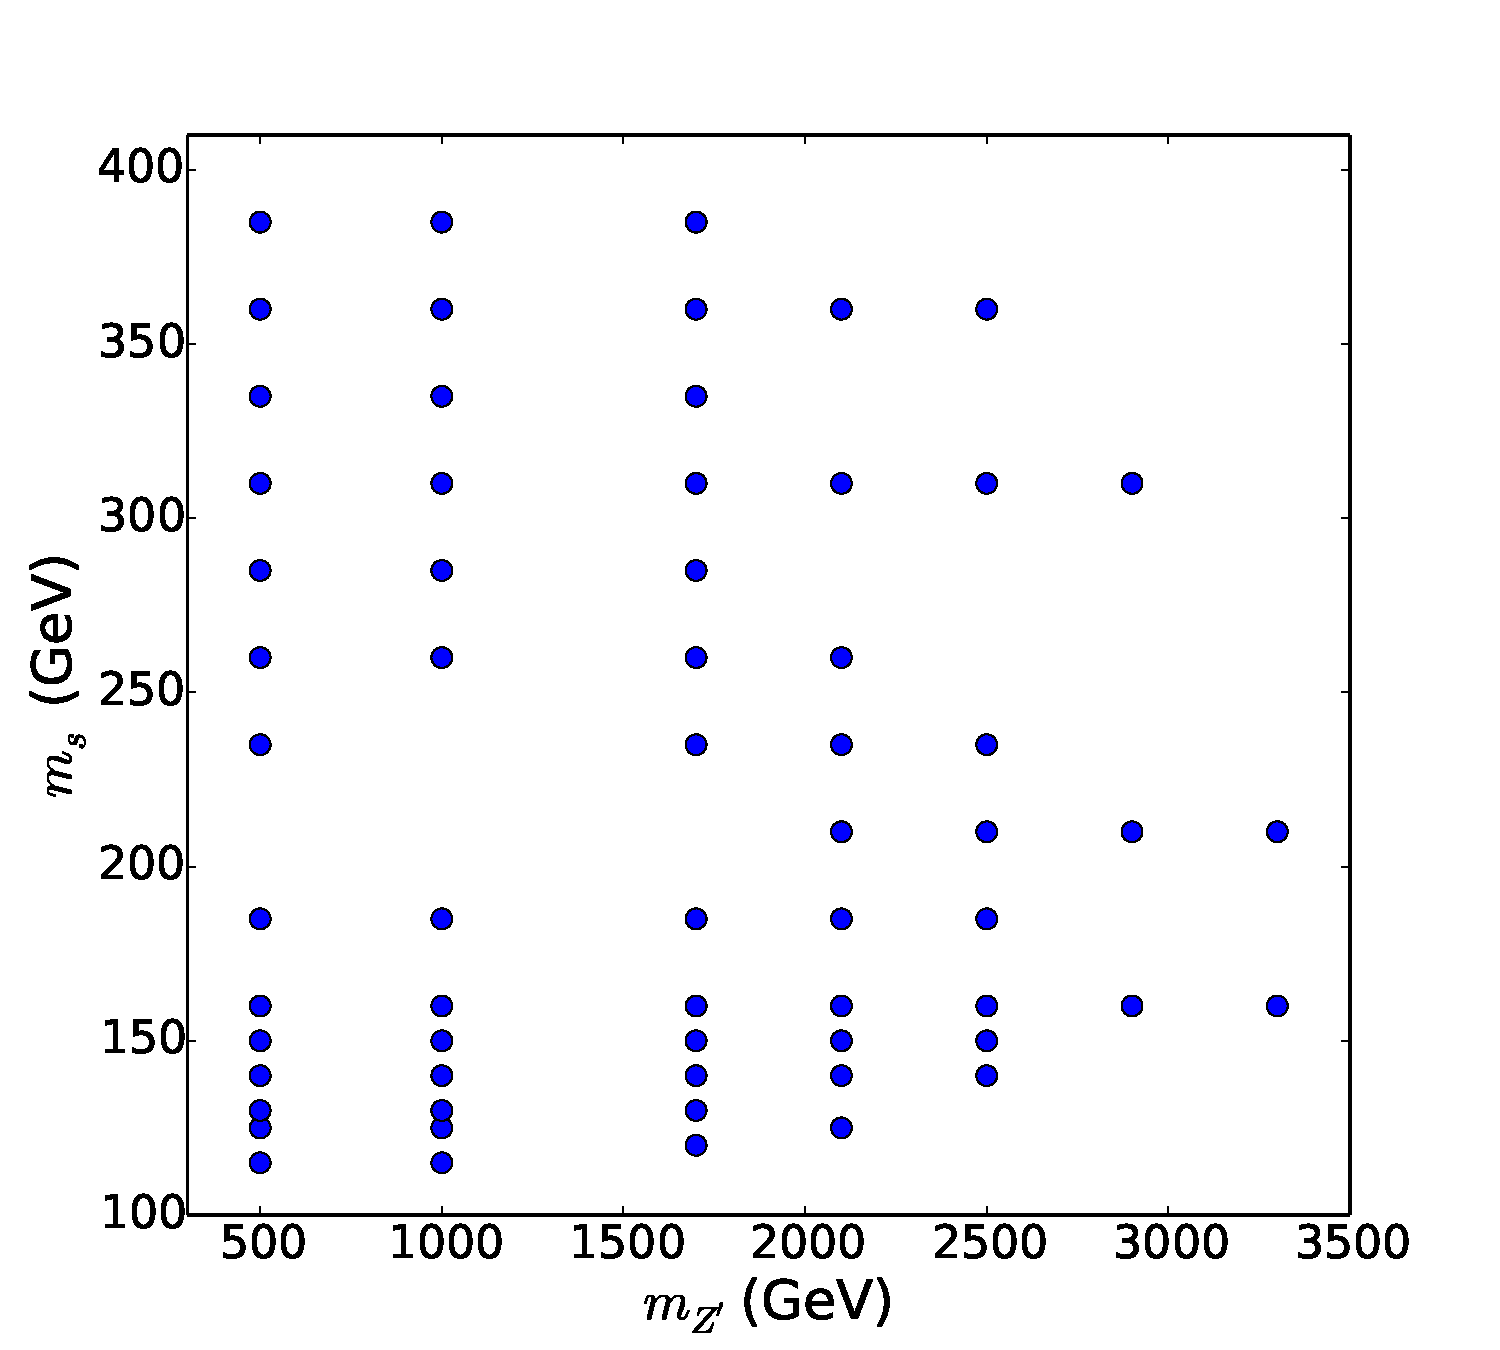
\includegraphics[width=0.8\textwidth]{Figures/4/Grid.pdf}
	\caption{Grid of produced signal samples with different choices of \mZp, \ms and the other parameters fixed to \(g_{q}=0.25\), \(g_{\chi} = 1.0\), \mchi = 200 GeV, \(\theta = 0.01\).}
	\label{fig:signalgrid}
\end{figure}

As discussed in Chapter \ref{chapter:dh_model}, the signal model considered in this search produces two final-state partons from the \(s \rightarrow WW(qq\ell\nu\)) decay. MadGraph also includes production mechanisms in the matrix element calculation for which up to one additional parton is radiated in the final state. These final-state partons initiate cascades of radiation produced by QCD processes \cite{parton_shower}, which are modelled using the Pythia8\footnote{The \PYTHIA[8.230]\cite{Sjostrand:2014zea} is the particular version of Pythia8 used to generate the MC simulated signal events used in this search.} program.

\section{Simulation of SM Background Processes}
\label{sec:SM_bkg_sim}

The selection criteria applied to final-state observables in the ATLAS and MC simulated events are designed to define signal regions which contain events that exhibit the final-state signature of the DH signal model, namely of a \(WW\) pair which decays semileptonically and which recoils against missing transverse momentum produced by the dark matter pair in the final state. However, some SM processes can produce final state observables which are similar enough to that of the signal model as to create an appreciable yield of events in the signal regions. In addition to targeting the signal model, the selections are also optimized to minimize the predicted yield of SM background processes in the signal regions. This section presents the background processes which have a non-negligible yield in the signal regions even with the optimized signal region selections.

Dominant backgrounds to the search are the \wjets, Diboson and \ttbar processes described in Section \ref{sec:dominant_bkgs}. 
%The \wjets and \ttbar processes are estimated by MC simulation in combination with the use of data-driven control region to constrain the background normalization in the combined fit. Other backgrounds are estimated purely by simulation.
Figure \ref{fig:background_yield_breakdown} shows the yield breakdowns in the signal regions of all SM background processes considered in the analysis.

\begin{figure}[h]
  \centering
     \begin{subfigure}{0.49\textwidth}
     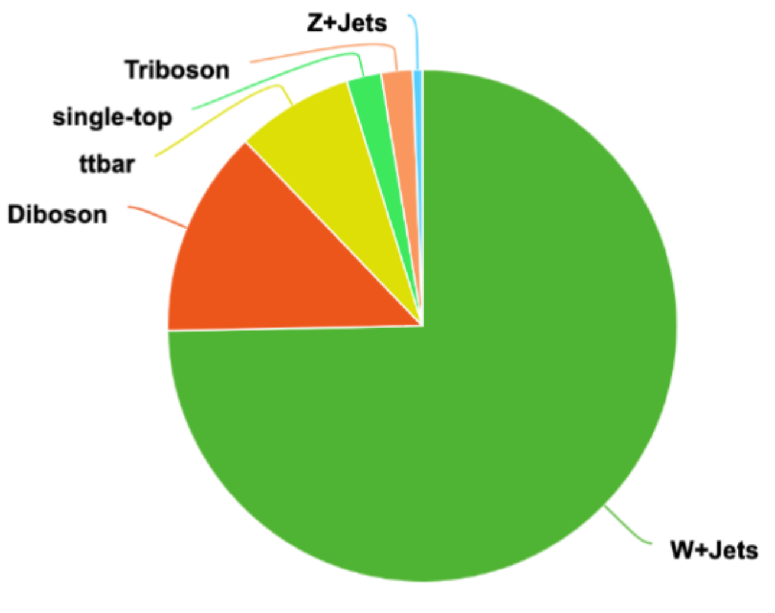
\includegraphics[width = 0.98\textwidth]{Figures/4/background_yield_breakdown_merged_SR.pdf}
    \caption{\merged SR}
    \label{fig:background_yield_breakdown_merged_SR}
     \end{subfigure}
    \begin{subfigure}{0.49\textwidth}
     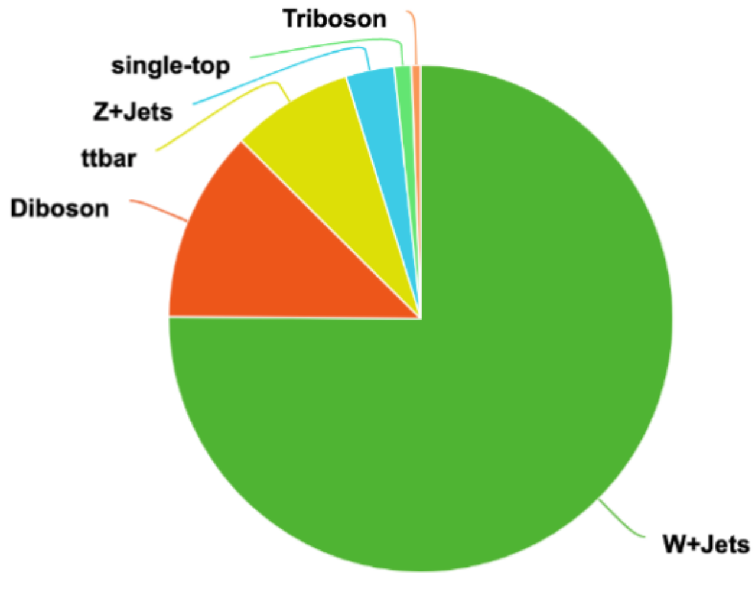
\includegraphics[width = 0.98\textwidth]{Figures/4/background_yield_breakdown_resolved_SR.pdf}
     \caption{\resolved SR}
     \label{fig:background_yield_breakdown_resolved_SR}
     \end{subfigure}
     \caption{Relative contribution of all SM background processes considered in the signal regions}
     \label{fig:background_yield_breakdown}
  \end{figure}


\subsection{Dominant Background Processes}
\label{sec:dominant_bkgs}

\subsubsection{W+jets}
\label{sec:wjets_description}

The dominant SM background in the signal regions comes from the \wjets process, wherein a leptonically decaying \(W\) is produced from the initial parton-parton collision, along with hadronic activity which fakes the hadronically decaying \(W\) in the signal model. A leading Feynman diagram for the \wjets background is shown in Figure \ref{fig:Wjets_Feynman}.

\begin{figure}[h]
  \centering
     \begin{subfigure}{0.49\textwidth}
     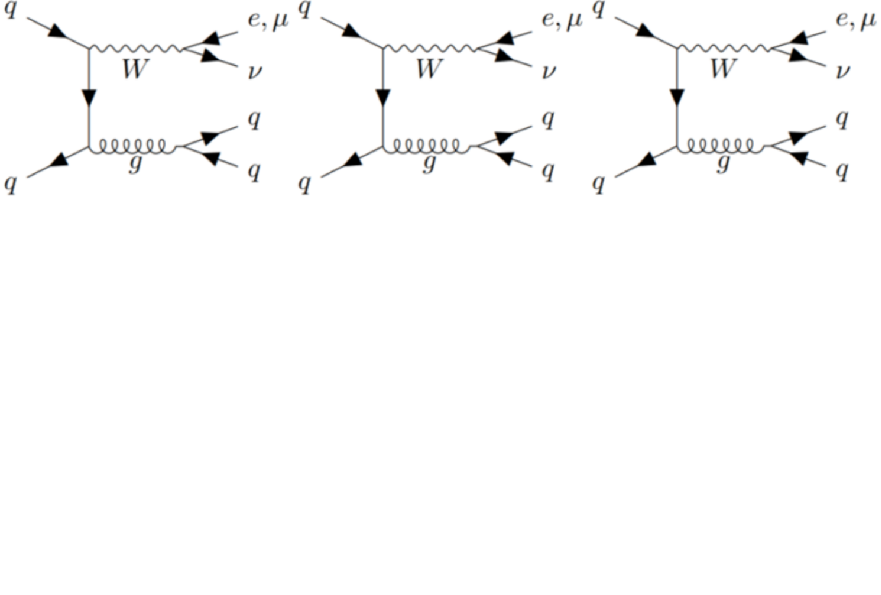
\includegraphics[width = 0.75\textwidth]{Figures/4/Fey_Wjets.pdf}
    \caption{\wjets}
    \label{fig:Wjets_Feynman}
     \end{subfigure}
    \begin{subfigure}{0.49\textwidth}
     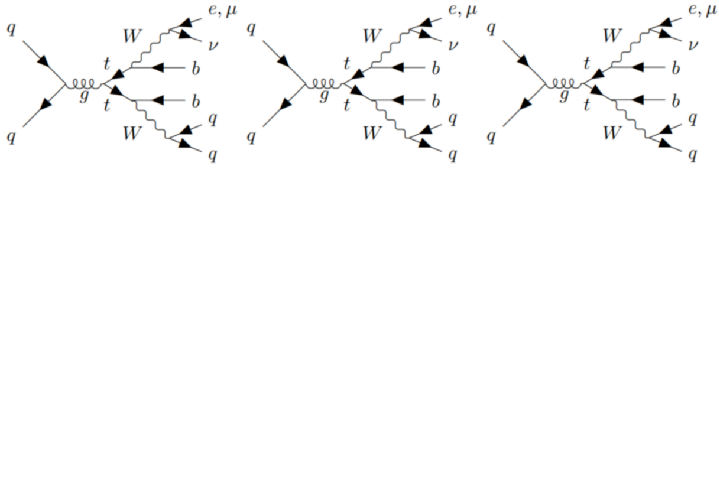
\includegraphics[width = 0.75\textwidth]{Figures/4/Fey_ttbar.pdf}
     \caption{\ttbar}
     \label{fig:ttbar_Feynman}
     \end{subfigure}
     \caption{Feynman diagrams for \wjets and \ttbar SM background processes}
     \label{fig:Feynman_bkgs}
  \end{figure}
  
The \SHERPA[2.2]~\cite{Gleisberg:2008ta} MC generator is used to model both the hard \wjets process, as well as the parton shower initiated by the final-state partons in the process. 

\medskip\noindent\textbf{Statistical Enhancement in \wjets Samples for \(m_W>120~\GeV\)}

Due to application of a high \mtlepmet requirement, described in Section \ref{sec:evt_selections} \textcolor{red}{(Note to Bob: section is not yet written)}, to reduce the \wjets background in the signal region, it was found that the majority of MC simulated events simulated for the \wjets process which make it into the signal regions are generated with a very high off-shell mass of the leptonically decaying \(W\) boson in the process \textcolor{red}{(Note to Bob/self: will need to discuss the concept of virtual and on-/off-shell production in Ch. 1)}. The default \SHERPA[2.2] generator is not optimized to produce large MC statistics in this high-\(m_W\) regime. Therefore, in addition to using samples produced by the default \SHERPA[2.2] generator, this search also makes use of a recently-developed set of specialized \SHERPA[2.2] \wjets MC generated samples\footnote{The specialized samples generated with enhanced MC statistics for large off-shell \(m_W\) are not yet discussed in any published work, but are described in the following internal ATLAS document: \href{https://cds.cern.ch/record/2753199}{ATL-COM-PHYS-2021-063}} that are generated with enhanced MC statistics for large off-shell masses (\(m_W > 120~\GeV\)) of the leptonically decaying \(W\).

\subsubsection{Diboson}
\label{sec:diboson_description}

The next-leading SM background after \wjets comes from the diboson process in which a pair of vector bosons - \(WW\), \(ZZ\) or \(WZ\) - are produced from the initial parton-parton collision. The diboson events which make it into the signal region are dominated by the production mechanism in which both bosons decay leptonically (\(W \rightarrow \ell\nu\), \(Z \rightarrow \nu\nu\) or \(Z \rightarrow \ell\ell\)) to produce a final-state lepton in addition to missing transverse momentum from the neutrino production, and one or more partons are radiated as part of the diboson production process to produce QCD activity which fakes the hadronically decaying \(W\) in the signal model. 

The diboson process, as well as the parton showers initiated by partons produced in the process, is modelled using the \SHERPA[2.2] MC generator. 

\subsubsection{\(\mathbf{t\bar{t}}\)}
\label{sec:ttbar_description}

The \ttbar process represents the third-leading SM background in the signal regions. A leading Feynman diagram for the process is shown in Figure \ref{fig:ttbar_Feynman}. In this process, two \(t\) quarks are produced from the initial parton-parton collision, both of which decay to a \(b\) quark and a \(W\) boson. The \(WW\) pair decays semileptonically, thus faking the semileptonically decaying \(WW\) pair produced in the signal model. The final-state \(\nu\) from the leptonic \(W\) decay produces the missing transverse momentum required in the signal region selection. The signal region selection includes a veto on the presence of \(b\)-tagged quarks in the final state to reduce the yield of \ttbar events, but some events from the process pass the veto and make it into the signal region due to the limited efficiency of the \(b\) quark tagging algorithm \cite{Varni:2742644}.

The production of \ttbar events is modelled using the \POWHEGBOX~v2~\cite{Frixione:2007nw,Nason:2004rx,Frixione:2007vw,Alioli:2010xd} generator which calculates matrix elements for the process. Parton showers initiated by final-state partons produced in the \ttbar process are modelled using \PYTHIA8.230~\cite{Sjostrand:2014zea}. 

\subsection{Sub-dominant Background Processes}

\subsubsection{Z+jets}
\label{sec:zjets_description}

The \zjets process is analogous to the \wjets process, but with the leptonically decaying \(W\) boson replaced by a \(Z\) boson, which also decays leptonically. For the majority of \zjets events which are classified into the signal region, the \(Z\) boson decays to a \(\ell\ell\) pair, of which one of the \(\ell\)s is not properly identified as a \(e\) or \(\mu\) during event reconstruction. 

\subsubsection{Triboson}
\label{sec:triboson_description}

The triboson process is similar in structure to the diboson, except that three vector bosons rather than two are produced from the initial parton-parton collision. Triboson events which pass the signal region selection predominantly exhibit a ``\(VVjj\)" final state in which two of the vector bosons decay leptonically to produce a final-state \(e\) or \(\mu\) in addition to missing transverse momentum from \(\nu\) production, and the third vector boson decays hadronically. The triboson process, as well as parton showers initiated by final-state partons in the process, is modelled using the \SHERPA[2.2] MC generator. 

\subsubsection{single-top}
\label{sec:stop_description}

The single-top process in the signal region is dominated by ``\(Wt\)" events \cite{stopWt} in which a single \(t\) quark is produced in association with a \(W\) boson from the initial collision of a quark and a gluon. The \(t\) quark subsequently decays to \(Wb\) to produce the signature \(WW\) final state of the signal model. As with the \ttbar background, the yield of single-top events in the signal region is reduced by the application of a \(b\)-veto in the event selection for the signal region.    

Single-top \(Wt\) associated production is modelled using the \POWHEGBOX~\cite{Re:2010bp,Nason:2004rx,Frixione:2007vw,Alioli:2010xd}~v2 generator which provides matrix elements for the process. Parton showers initiated by final-state partons produced in the single-top \(Wt\) process are modelled using \PYTHIA8.230~\cite{Sjostrand:2014zea}. 

